\documentclass[10pt]{article}
\usepackage{zsj}

\usepackage{silence}
\WarningFilter{latex}{Marginpar on page}

\allowdisplaybreaks

\hbadness=99999

\newcommand{\me}{\mathrm{e}}
%\newcommand{\rr}{\mathbb{R}}
\newcommand{\ii}{\mathrm{i}}
%\newcommand{\md}{\mathrm{d}}
%\DeclareMathOperator{\im}{im}


\usepackage{annotate-equations}
\usepackage{marginfix}


\newenvironment{boxmath}[1]{\begin{tcolorbox}[enhanced,attach boxed title to top center={yshift=-\tcboxedtitleheight/2},boxrule=1pt,title={\centering #1},colframe=NavyBlue!70!black,colback=NavyBlue!10,colbacktitle=NavyBlue!10,fonttitle=\scshape,coltitle=Black]}{\end{tcolorbox}}
\crefname{claim}{claim}{claims}


\begin{document}
\title{Conformal Field Theory}
\subheader{Notes}
\author{Shangjie Zhou\orcidlink{0000-0001-9576-5011}}
\affiliation{School of Physics and Technology, Wuhan University}
\emailAdd{sjzhou@whu.edu.cn}
\abstract{\textit{Last updated on: \today}\\Repository: \url{https://github.com/spaceofzsj/Notes}\\Personal Website: \url{https://spaceofzsj.github.io/ShangjieZhou/}\\Blog: \url{https://spaceofzsj.github.io/}}
\maketitle
\section*{Introduction}
\addcontentsline{toc}{section}{\protect\numberline{}Introduction}
A conformal field theory (CFT) is a quantum field theory that is invariant under \textit{conformal transformations}.

Conformal field theory has important applications to condensed matter physics, statistical mechanics, quantum statistical mechanics, and string theory.

This notes are mainly based on \cite{DiFrancesco:1997nk}.

There are also useful lecture notes like \cite{Qualls:2015qjb,Tong:2009np}.

\clearpage
\part{Review}
\section{Quantum Field Theory}
\subsection{Symmetries and Conservation Laws}
\subsubsection{Continuous Symmetry Transformations}
Consider a collection of fields, which are denoted by $\Phi(x)$.
The action is
\begin{align}
    S=\int\dd[d]{x}\mathcal{L}\left(\Phi,\partial_\mu\Phi\right).
\end{align}
Consider a transformation affecting both the position and the field
\begin{subequations}\label{eq:CST:transformations}
    \begin{align}
        x       & \to x'       \\
        \Phi(x) & \to\Phi'(x')
    \end{align}
\end{subequations}
In the transformations \cref{eq:CST:transformations}, the new field $\Phi'$ at $x'$ is expressed as a function of the old field $\Phi$ at $x$
\begin{align}
    \Phi'(x')=\mathcal{F}\left(\Phi(x)\right).
\end{align}
\begin{figure}[h]
    \centering
    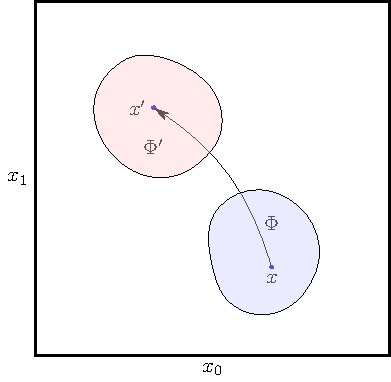
\includegraphics[width=0.5\linewidth]{fig/Quantum Field Theory/transformation_illustration/fig.pdf}
    \caption{A illustration of the transformation of the fields where the background spacetime is 2-dimensional. The colored areas are the non-vanishing part of the fields.}
\end{figure}

The new action is
\begin{align}
    S' & =\int\dd[d]{x}\mathcal{L}\left(\Phi'(x),\partial_\mu\Phi'(x)\right)\notag                                                                                               \\
       & =\int\dd[d]{x'}\mathcal{L}\left(\Phi'(x'),\partial'_\mu\Phi'(x')\right)\notag                                                                                           \\
       & =\int\dd[d]{x'}\mathcal{L}\left(\mathcal{F}\left(\Phi(x)\right),\partial'_\mu\mathcal{F}(\Phi(x))\right)\notag                                                          \\
       & =\int\dd[d]{x}\abs{\pdv{x'}{x}}\mathcal{L}\left(\mathcal{F}(\Phi(x)),\left(\pdv*{x^\nu}{x'^\mu}\right)\partial_\nu\mathcal{F}(\Phi(x))\right).\label{eq:CST:new_action}
\end{align}
\subsubsection{Infinitesimal Transformations and Noether's Theorem}
Infinitesimal transformations may in general written as
\begin{align}
    x'^\mu    & =x^\mu+\omega_a\fdv{x^\mu}{\omega_a}\label{eq:CST:x_prime}               \\
    \Phi'(x') & =\Phi(x)+\omega_a \fdv{\mathcal{F}(x)}{\omega_a}\label{eq:CST:phi_prime}
\end{align}
Here $\{\omega_a\}$ is a set of infinitesimal parameters, which will be kept to first order only.
\begin{definition}[Generator of a symmetry transformation]\label{def:generator_of_a_symmetry_transformation}
    The \textit{generator} $G_a$ of a symmetry transformation is defined by the following expression for the infinitesimal transformation at a same point:
    \begin{align}
        \delta_\omega\Phi(x)\equiv\Phi'(x)-\Phi(x)\equiv-\ii\omega_a G_a\Phi(x).
    \end{align}
\end{definition}
Notice that
\begin{align}
    \Phi'(x')=\Phi(x)+\omega_a \fdv{\mathcal{F}(x)}{\omega_a}=\Phi(x')-\omega_a\fdv{x^\mu}{\omega_a}\partial_\mu\Phi(x')+\omega_a\fdv{\mathcal{F}(x')}{\omega_a}
\end{align}
The explicit expression of the generator is therefore
\begin{align}
    \ii G_a\Phi=\fdv{x^\mu}{\omega_a}\partial_\mu\Phi-\fdv{\mathcal{F}}{\omega_a}\label{eq:CST:explicit_generator}
\end{align}
\begin{example}[Infinitesimal translation]
    For an infinitesimal translation by a vector $\omega_\mu$, one has $\fdv*{x^\mu}{\omega^\nu}=\delta^\mu_\nu$ and $\fdv*{\mathcal{F}}{\omega^\nu}=0$.
    The generator of translations is simply
    \begin{align}
        P_\nu=-\ii\partial_\nu.
    \end{align}
\end{example}
\begin{example}[Infinitesimal Lorentz transformation]
    An infinitesimal Lorentz transformation has the form
    \begin{align}
        x'^\mu=x^\mu+\tensor{\omega}{^\mu_\nu}x^\nu=x^\mu+\omega_{\rho\nu}\eta^{\rho\mu}x^\nu.
    \end{align}
    where $\omega_{\rho\nu}=-\omega_{\nu\rho}$.
    Thus the variation of coordinates under transformation is
    \begin{align}
        \fdv{x^\mu}{\omega_{\rho\nu}}=\frac{1}{2}\left(\eta^{\rho\mu}x^\nu-\eta^{\nu\mu}x^\rho\right).\label{eq:CST:lorentz_x}
    \end{align}
    And its effect on the generic field $\Phi$ is
    \begin{align}
        \mathcal{F}(\Phi)=L_\Lambda \Phi\qq{and}L_\Lambda\approx1-\frac{1}{2}\ii\omega_{\rho\nu}S^{\rho\nu}\label{eq:CST:lorentz_phi}
    \end{align}
    where  $S^{\rho\nu}$ is some Hermitian matrix obeying the Lorentz algebra.
    Using \cref{eq:CST:explicit_generator}, we have
    \begin{align}
        \frac{1}{2}\ii\omega_{\rho\nu}L^{\rho\nu}\Phi=\frac{1}{2}\omega_{\rho\nu}\left(x^\nu\partial^\rho-x^\rho\partial^\nu\right)\Phi+\frac{1}{2}\ii\omega_{\rho\nu}S^{\rho\nu}\Phi
    \end{align}
    The generators of the Lorentz transformation are thus
    \begin{align}
        L^{\rho\nu}=\ii\left(x^\rho\partial^{\nu}-x^\nu\partial^\rho\right)+S^{\rho\nu}.
    \end{align}
\end{example}
\begin{theorem}[Noether's theorem]
    Every continuous symmetry of the action is associated with a current that is \textit{classically}\snm conserved.
\end{theorem}
\snt{Notice the \textit{classically}. In the quantum case, it may happen that the path integration measure does not possess the symmetry of the action, in which case that symmetry is said to be \textit{anomalous}.}
\begin{proof}
    Using \cref{eq:CST:x_prime,eq:CST:phi_prime} in \cref{eq:CST:new_action}, we have
    \begin{align}
        \pdv{x'^\mu}{x^\mu}=\delta^\nu_\mu+\partial_\mu\left(\omega_a\fdv{x^\nu}{\omega_a}\right).\label{eq:qft:infinitesimal_inverse}
    \end{align}
    Using the first order approximation of the determinant of a matrix
    \begin{align}
        \det(1+E)\approx1+\Tr E\quad(E\ \text{is small})
    \end{align}
    we have
    \begin{align}
        \abs{\pdv{x'}{x}}\approx1+\partial_\mu\left(\omega_a\fdv{x^\mu}{\omega}\right)
    \end{align}
    and the reverse of \cref{eq:qft:infinitesimal_inverse} is
    \begin{align}
        \pdv{x^\nu}{x'^\mu}=\delta^\nu_\mu-\partial_\mu\left(\omega_a\fdv{x^\nu}{\omega_a}\right).
    \end{align}
    Now \cref{eq:CST:new_action} becomes
    \begin{align}
        S'= & \int\dd[d]{x}\left(1+\partial_\mu\left(\omega_a\pdv{x^\mu}{\omega_a}\right)\right)\notag                                                                                                                                                             \\
            & \times\mathcal{L}\left(\Phi+\omega_a\pdv{\mathcal{F}}{\omega_a},\left[\delta^\nu_\mu-\partial_\mu\left(\omega_a\fdv{x^\nu}{\omega_a}\right)\right]\left[\partial_\nu\Phi+\partial_\nu\left(\omega_a\fdv{\mathcal{F}}{\omega_a}\right)\right]\right).
    \end{align}
    From the definition of symmetry, when $\omega_a$ are constants the variation $\delta S$ vanishes.
    So $\delta S$ can only contain first derivatives of $\omega_a$, obtained by expanding the Lagrangian\snm,
    \begin{align}
        \delta S\equiv S'-S=-\int\dd[d]{x}j^\mu_a\partial_\mu\omega_a\label{eq:nother:before_integration}
    \end{align}
    where
    \begin{align}
        j^\mu_a\equiv\left(\pdv{\mathcal{L}}{(\partial_\mu\Phi)}\partial_\nu\Phi-\delta^\mu_\nu\mathcal{L}\right)\fdv{x^\nu}{\omega_a}-\pdv{\mathcal{L}}{(\partial_\mu\Phi)}\fdv{\mathcal{F}}{\omega_a}.\label{eq:nother:canonical_current}
    \end{align}
    $j^\mu_a$ is called the \textit{current} associated with the infinitesimal transformation.
    Integrate \cref{eq:nother:before_integration} by parts
    \begin{align}
        \delta S=\int\dd[d]{x}\partial_\mu j^\mu_a \omega_a.
    \end{align}
    When the field configuration obeys the classical equation of motion, $\delta S=0$ for any postion-dependent parameters $\omega_a(x)$, which implies the conservation law
    \begin{align}
        \partial_\mu j^\mu_a=0.
    \end{align}
    The conserved charge associated with $j^\mu_a$ is
    \begin{align}
        Q_a\equiv\int\dd[d-1]{x}j^0_a.
    \end{align}
    We can show that
    \begin{align}
        \dot{Q}_a= & \int\dd[d-1]{x}\partial_0 j^0_a\notag                            \\
        =          & -\int\dd[d-1]{x}\partial_i j^i_a\label{eq:nother:stocks_theorem} \\
        =          & -\int_\infty j^i_a\dd{\sigma^i}\notag                            \\
        =          & 0
    \end{align}
    where we used Stokes' theorem in \cref{eq:nother:stocks_theorem} and $\dd{\sigma^i}$ is the turface element at spatial infinity.
\end{proof}
\snt{This is where the symmetry condition is used: when the transformation is not a symmetry transformation, if $\omega_a$ is constant then $\delta S$ may not vanish, and the expansion must involve terms without derivative; when the transformation is a symmetry transformation, if $\omega_a$ is constant then $\delta S=0$, so it is reasonable there are only terms with derivatives in $\delta S$ and all the terms without derivatives must sum up to $0$. After expanding $\delta S$, we find that that there is only term with first derivative.}
\begin{remark}
    We can freely add $j^\mu_a$ the divergence of an antisymmetric tensor without affecting the conservation
    \begin{align}
        j^\mu_a\to j^\mu_a+\partial_\nu B^{\nu\mu}_a\qq{where} B^{\nu\mu}_a=-B^{\mu\nu}_a
    \end{align}
    since $\partial_\mu\partial_\nu B^{\nu\mu}_a=0$ by antisymmetry.
    The current we defined in \cref{eq:nother:canonical_current} is said to be \textit{canonical}.
\end{remark}
\subsubsection{Transformations of the Correlation Functions}
Consider the general correlation function
\begin{align}
    \expval{\Phi(x_1)\dots\Phi(x_n)}=\frac{1}{\eqnmarkbox[blue]{node1}{Z}}\int\left[\dd{\Phi}\right]\Phi(x_1)\dots\Phi(x_n)\exp(-\eqnmarkbox[purple]{node2}{S[\Phi]})
\end{align}
\annotate[yshift=-0.1em]{below}{node1}{Vacuum functional}
\annotate[yshift=0.5em]{}{node2}{Euclidean action}

When the transformation \cref{eq:CST:transformations} is a symmetry, we have the following constraint on the correlation function
\begin{subequations}\label{eq:TCF:correlation_transform}
    \begin{align}
        \expval{\Phi(x_1')\dots\Phi(x_n')}= & \frac{1}{Z}\int\left[\dd{\Phi}\right]\Phi(x_1')\dots\Phi(x_n')\exp(-S(\Phi))\notag                                                                  \\
        =                                   & \frac{1}{Z}\int\left[\dd{\Phi'}\right]\Phi'(x_1')\dots\Phi'(x_n')\exp(-S(\Phi'))\label{eq:TCF:measure1}                                             \\
        =                                   & \frac{1}{Z}\int\left[\dd{\Phi}\right]\mathcal{F}\left(\Phi(x_1')\right)\dots\mathcal{F}\left(\Phi(x_n')\right)\exp(-S(\Phi))\label{eq:TCF:measure2} \\
        =                                   & \expval{\mathcal{F}\left(\Phi(x_1)\right)\dots\mathcal{F}\left(\Phi(x_n)\right)}
    \end{align}
\end{subequations}
We have assumed the Jacobian of this change of variable is trivial in \crefrange{eq:TCF:measure1}{eq:TCF:measure2}\sidenote{This is in fact the main obstacle to conformal invariance in a quantum symmetry: the action may well be scale invariant, but the measure is not because of the regularization procedure needed to define it properly.}.

\subsubsection{Ward Identities}
We can write the \textit{global} infinitesimal transformation as

\begin{align}
    \Phi'(x)=\Phi(x)-\ii\eqnmarkbox[blue]{node1}{\omega_a} G_a\Phi(x).
\end{align}\annotate[yshift=0.5em]{}{node1}{Infinitesimal constant parameters}

Now we consider the \textit{local} infinitesimal transformation in which parameters will depend on spacetime coordinates
\begin{align}
    \Phi'(x)=\Phi(x)-\ii\omega_a(x) G_a\Phi(x).
\end{align}
Denoting by $X$ and $X'$ the collection $\Phi(x_1)\dots\Phi(x_n)$ and $\Phi'(x_1)\dots\Phi'(x_n)$ of fields in the correlation function respectively and by $\delta_\omega X\equiv X'-X$ its variation under the transformation, we can do a change of variable
\begin{align}
    \expval{X}= & \frac{1}{Z}\int\left[\dd{\Phi}\right]X\exp(-S[\Phi])\notag                                                                                                                       \\
    =           & \frac{1}{Z}\int\left[\dd{\Phi'}\right]X'\exp(-S[\Phi'])\notag                                                                                                                    \\
    =           & \frac{1}{Z}\int\left[\dd{\Phi}\right]\left(X+\delta_\omega X\right)\exp\left[-\left(S[\Phi]+\int\dd[d]{x}\partial_\mu j^\mu_a\omega_a(x)\right)\right]\label{eq:ward:before_est}
\end{align}
where we have used \cref{eq:nother:before_integration} and assuemd the functional integration measure is invariant under the transformation $\left[\dd{\Phi'}\right]=\left[\dd[]{\Phi}\right]$.
Expand \cref{eq:ward:before_est} to first order in $\omega_a(x)$, we have
\begin{align}
    \expval{X} & =\frac{1}{Z}\int\left[\dd[]{\Phi}\right]\left(X+\delta_\omega X\right)\exp(-S)\left[1-\int\dd[]{x}\partial_\mu j^\mu_a\omega_a(x)\right]\notag \\
               & =\expval{X}+\expval{\delta_\omega X}-\int\dd[d]{x}\partial_\mu\expval{j^\mu_a(x)X}\omega_a(x)
\end{align}
which finally gives\sidenote{It is clearly that $$\expval{\delta_\omega X}=\delta_\omega\expval{X}.$$}
\begin{align}
    \expval{\delta_\omega X}=\int\dd[d]{x}\partial_\mu\expval{j^\mu_a(x)X}\omega_a(x).\label{eq:ward:anyomega}
\end{align}
The variation $\delta_\omega X$ is explicitly given to first order in $\omega_a(x)$ by
\begin{align}
    \delta_\omega X & =-\ii\sum_{i=1}^n\left(\Phi(x_1)\dots G_a\Phi(x_i)\dots\Phi(x_n)\right)\omega_a(x_i)\notag                    \\
                    & =-\ii\int\dd[d]{x}\omega_a(x)\sum_{i=1}^n\left[\Phi(x_1)\dots G_a\Phi(x_i)\dots\Phi(x_n)\right]\delta(x-x_i).
\end{align}
Since \cref{eq:ward:anyomega} holds for any $\omega_a(x)$, we have the local relation which is called the \textit{Ward identity} for the current $j^\mu_a$.
\begin{boxmath}{Ward Identity}
    \begin{align}
        \pdv{x^\mu}\expval{j^\mu_a(x)\Phi(x_1)\dots\Phi(x_n)}=-\ii\sum^n_{i=1}\delta(x-x_i)\expval{\Phi(x_1)\dots G_a\Phi(x_i)\dots\Phi(x_n)}.\label{eq:QFT:ward_identity}
    \end{align}
\end{boxmath}
\begin{remark}
    The form of the current may be modified from the canonical definition \cref{eq:nother:canonical_current} without affecting the Ward identity, if we add a term to $j^\mu_a$ that is divergenceless identically.
\end{remark}
\subsection{The Energy-Momentum Tensor}
The conserved current associated with translation invariance is the \textit{energy-momentum tensor}, whose components are the density and flux density of energy and momentum.

Consider the infinitesimal translation\sidenote{The field is unaffected by the translation.} $x^\mu\to x^\mu+\epsilon^\mu$, we have
\begin{align}
    \fdv{x^\mu}{\epsilon^\mu}=\delta^\mu_\nu\quad\fdv{\mathcal{F}(x)}{\epsilon^\mu}=0.
\end{align}
Using \cref{eq:nother:canonical_current}, the corresponding canonical conserved current is
\begin{align}
    T^{\mu\nu}_c\equiv-\eta^{\mu\nu}\mathcal{L}+\pdv{\mathcal{L}}{(\partial_\mu\Phi)}\partial^\nu\Phi
\end{align}
which satisfies
\begin{align}
    \partial_\mu T^{\mu\nu}_c=0.
\end{align}
The conserved charge is the 4-momentum
\begin{align}
    P^\nu\equiv\int\dd[d-1]{x}T^{0\nu}_c.
\end{align}
In particular, the energy is
\begin{align}
    P^0=\int\dd[d-1]{x}\left(\pdv{\mathcal{L}}{\dot{\Phi}}\dot{\Phi}-\mathcal{L}\right)
\end{align}
which is the usual definition of the Hamiltonian.

\subsubsection{The Belinfante Tensor}
\begin{intu}
    In general, the canonical energy-momentum operator is not symmetric, we can make it symmetric by adding $T^{\mu\nu}_c$ an divergenceless term without breaking the consevation law or the Ward identity
    \begin{align}
        T^{\mu\nu}_B=T^{\mu\nu}_c+\partial_{\rho}B^{\rho\mu\nu}\qq{where}B^{\rho\mu\nu}=-B^{\mu\rho\nu}.
    \end{align}
\end{intu}
The variation of the action under a nonuniform translation with position-dependent parameter $\epsilon^\mu(x)$ is still
\begin{align}
    \delta S=-\int\dd[d]{x}\partial_\mu T^{\mu\nu}_B\epsilon_\nu
\end{align}
since $\partial_\mu T^{\mu\nu}_B=\partial_\mu T^{\mu\nu}_c$.

If we succeed in finding $B^{\rho\mu\nu}$ such that the new tensor $T^{\mu\nu}_B$ is symmetric, then the latter is called the \textit{Belinfante} energy-momentum tensor.

\paragraph{Finding Belinfante tensor}
From \cref{eq:CST:lorentz_x,eq:CST:lorentz_phi}, under infinitesimal Lorentz transformation, the coordinates and fields change as
\begin{align}
    \fdv{x^\rho}{\omega_{\mu\nu}}=\frac{1}{2}\left(\eta^{\rho\mu}x^\nu-\eta^{\rho\nu}x^\mu\right)\qand\fdv{\mathcal{F}}{\omega_{\mu\nu}}=-\frac{\ii}{2}S^{\mu\nu}\rho
\end{align}
and the associated conserved current is
\begin{align}
    j^{\mu\nu\rho}=T^{\mu\nu}_c x^\rho-T^{\mu\rho}_c x^\nu+\frac{\ii}{2}\pdv{\mathcal{L}}{(\partial_\mu\Phi)}S^{\nu\rho}\Phi.\label{eq:Belinfante:lorentz_current}
\end{align}
\begin{claim}
    One of the possible form of $B^{\rho\mu\nu}$ that will make $T^{\mu\nu}_B$ symmetric is
    \begin{align}
        B^{\mu\rho\nu}=\frac{\ii}{4}\left[\pdv{\mathcal{L}}{(\partial_\mu\Phi)}S^{\nu\rho}\Phi+\pdv{\mathcal{L}}{(\partial_\rho\Phi)}S^{\mu\nu}\Phi+\pdv{\mathcal{L}}{(\partial_\nu\Phi)}S^{\mu\rho}\Phi\right].\label{eq:Belinfante:B}
    \end{align}
\end{claim}
\begin{proof}
    Using the fact $S^{\mu\nu}=-S^{\nu\mu}$, it can be easily checked that $B^{\mu\rho\nu}=-B^{\rho\mu\nu}$.

    We can explicitly show that
    \begin{align}
        B^{\mu\rho\nu}-B^{\mu\nu\rho}=\frac{1}{2}\ii\pdv{\mathcal{L}}{(\partial_\mu\Phi)}S^{\nu\rho}\Phi.
    \end{align}
    Acting $\partial_\mu$ on both sides of \cref{eq:Belinfante:lorentz_current}, we have
    \begin{align}
        T^{\rho\nu}_c-T^{\nu\rho}_c=-\frac{1}{2}\ii\partial_\mu\left[\pdv{\mathcal{L}}{(\partial_\mu\Phi)}S^{\nu\rho}\Phi\right]
    \end{align}
    where the conservation laws $\partial_\mu j^{\mu\nu\rho}=0$ and $\partial_\mu T^{\mu\nu}=0$ are used.
    We see that the antisymmetric part of $T^{\rho\nu}_c+\partial_\mu B^{\mu\rho\nu}$ vanishes which means $T^{\mu\nu}_B$ is indeed symmetric in a classical configuration.
\end{proof}
\begin{remark}
    The form of $B^{\mu\rho\nu}$ is not unique.
\end{remark}
\subsubsection{Alternate Definition of the Energy-Momentum Tensor}
Consider an infinitesimal translation of the coordinates $x^\mu\to x'^\mu+\epsilon^\mu(x)$.
According to \cref{eq:nother:before_integration}, we have
\begin{align}
    \delta S= & \int\dd[d]{x}T^{\mu\nu}\partial_\mu\epsilon_\nu\notag                                                                               \\
    =         & \frac{1}{2}\int\dd[d]{x}T^{\mu\nu}\left(\partial_\mu\epsilon_\nu+\partial_\nu\epsilon_\mu\right)\label{eq:alternate_tensor:delta_s}
\end{align}
where we have assumed $T^{\mu\nu}$ has been made symmetric.

The induced metric of the map $x^\mu\to x'^\mu+\epsilon^\mu(x)$ to first order in $\epsilon$ is
\begin{align}
    g'_{\mu\nu}= & \pdv{x^\alpha}{x'^\mu}\pdv{x^\beta}{x'^\nu}g_{\alpha\beta}\notag                                                                   \\
    =            & \left(\delta^\alpha_\mu-\partial_\mu\epsilon^\alpha\right)\left(\delta^\beta_\nu-\partial_\nu\epsilon^\beta\right)g_{\alpha\beta}.
\end{align}
\begin{intu}
    The form of the variation of the metric is a hint of a new definition of the energy-momentum tensor.
    We can rewrite \cref{eq:alternate_tensor:delta_s}
    \begin{align}
        \delta S=-\frac{1}{2}\int\dd[d]{x}T^{\mu\nu}\delta g_{\mu\nu}.
    \end{align}
\end{intu}
Therefore, we can give an alternate definition of the energy-momentum tensor
\begin{definition}[Alternate definition of energy-momentum tensor]
    The enery-momentum tensor is defined to be the functional derivative of the action with respect to the metric, evaluated in flat space:
    \begin{align}
        \delta S=-\frac{1}{2}\int\dd[d]{x}T^{\mu\nu}\delta g_{\mu\nu}.
    \end{align}
\end{definition}
\clearpage
\section{Statistical Mechanics}
\subsection{The Boltzmann Distribution}
\subsection{Critical Phenomena}
\subsection{The Renormalization Group: Lattice Models}
\subsection{The Renormalization Group: Continuum Models}
\subsection{The Transfer Matrix}
\clearpage
\part{Fundamentals}
\section{Global Conformal Invariance}
\subsection{The Conformal Group}
We denote by $g_{\mu\nu}$ the metric tensor in a spacetime of dimension $d$.
\begin{definition}[Conformal transformation]
    A conformal transformation of the coordinates is an invertible mapping $x\to x'$, for which the induced metric tensor invariant up to a scale:
    \begin{align}
        g'_{\mu\nu}(x')=\Lambda(x)g_{\mu\nu}(x).\label{eq:ct:conformal_transformation}
    \end{align}
\end{definition}
The induced metric can be calculated by
\begin{align}
    g'_{\mu\nu}(x')=\pdv{x^\rho}{x'^\mu}\pdv{x^\sigma}{x'^\nu}g_{\rho\sigma}(x).\label{eq:ct:induced_metric}
\end{align}
The set of conformal transformations manifestly forms a group, and it obviously has the Poincar\'{e} group as a subgroup, since the latter corresponds to the special case $\Lambda(x)=1$.
\subsubsection{Infinitesimal Conformal Transformation}
Consider an infinitesimal conformal transformation $x^\mu\to x'^{\mu}+\epsilon^\mu(x)$.
The induced metric is
\begin{align}
    g'_{\mu\nu}=g_{\mu\nu}-\left(\partial_\mu\epsilon_\nu+\partial_\nu\epsilon_\mu\right).
\end{align}
The requirement that the transformation be conformal implies that
\begin{align}
    \partial_\mu\epsilon_\nu+\partial_\nu\epsilon_\mu=f(x)g_{\mu\nu}.\label{eq:GCI:fx}
\end{align}
Taking the trace of both sides of \cref{eq:GCI:fx}, we have
\begin{align}
    f(x)=\frac{2}{d}\partial_\rho\epsilon^\rho.\label{eq:GCI:fx1}
\end{align}

For simplicity, we assume the original metric is standard Cartesian metric $g_{\mu\nu}=\eta_{\mu\nu}$, where $\eta_{\mu\nu}=\mathrm{diag}(1,1,\dots,1)$.\sidenote{Of cource we can consider Minkowski metric. The treatment is identical, except for the explicit form of $\eta_{\mu\nu}$.}
By applying an extra derivative $\partial_\rho$ on \cref{eq:GCI:fx}, permuting the indices and taking a linear combination, we arrive at
\begin{align}
    2\partial_\mu\partial_\nu\epsilon_\rho=\eta_{\mu\rho}\partial_\nu f+\eta_{\nu\rho}\partial_\mu f-\eta_{\mu\nu}\partial_\rho f.\label{eq:GCI:fx2}
\end{align}
Upon contracting with $\eta^{\mu\nu}$, \cref{eq:GCI:fx2} becomes
\begin{align}
    2\partial^2\epsilon_\mu=(2-d)\partial_\mu f \label{eq:GCI:fx3}
\end{align}
Applying $\partial_\nu$ on \cref{eq:GCI:fx3} and $\partial^2$ on \cref{eq:GCI:fx}, we have respectively
\begin{align}
    \partial^2\partial_\nu\epsilon_\mu= & \frac{2-d}{2}\partial_\mu\partial_\nu f\label{eq:GCI:fx4}                                \\
    \eta_{\mu\nu}\partial^2 f=          & \partial^2\partial_\mu\epsilon_\nu+\partial^2\partial_\nu\epsilon_\mu.\label{eq:GCI:fx5}
\end{align}
Combine \cref{eq:GCI:fx4,eq:GCI:fx5}, we have\sidenote{Notice that the $\mu$ and $\nu$ indices in \cref{eq:GCI:fx4} are symmetric.}
\begin{align}
    (2-d)\partial_\mu\partial_\nu f=\eta_{\mu\nu}\partial^2 f.\label{eq:GCI:fx6}
\end{align}
Finally, contracting \cref{eq:GCI:fx6} with $\eta^{\mu\nu}$, we end up with
\begin{align}
    (d-1)\partial^2 f=0.\label{eq:GCI:fx7}
\end{align}
\paragraph{The case $d=1$}
The above equations do not impose any constraint on the function $f$, and therefore any smooth transformation is conformal in one dimension.
\paragraph{The case $d=2$}
This case is special and it will be studied in detail later.
\paragraph{The case $d\geq3$}
Now \cref{eq:GCI:fx6,eq:GCI:fx7} imply that $\partial_\mu\partial_\nu f=0$ and therefore
\begin{align}
    f(x)=A+B_\mu x^\mu\label{eq:GCI:fxs}
\end{align}
where $A$ and $B_\mu$ are constants.
If we substitute \cref{eq:GCI:fxs} into \cref{eq:GCI:fx2}, we see that $\partial_\mu\partial_\nu\epsilon_\rho$ is constant, which means we have the general expression
\begin{align}
    \epsilon_\mu=a_\mu+b_{\mu\nu}x^\nu+c_{\mu\nu\rho}x^\nu x^\rho\qq{where}c_{\mu\nu\rho}=c_{\mu\rho\nu}.
\end{align}
$a_\mu$, $b_{\mu\nu}$ and $c_{\mu\nu\rho}$ are constants.
We can treat each power of the coordinate separately and use the constraints \cref{eq:GCI:fx,eq:GCI:fx1,eq:GCI:fx2}:
\begin{itemize}
    \item The constant term $a_\mu$ is free of constraints.
          This term amounts to an infinitesimal translation.
    \item Substitution of the linear term into \cref{eq:GCI:fx,eq:GCI:fx1} yields
          \begin{align}
              b_{\mu\nu}+b_{\nu\mu}=\frac{2}{d}\tensor{b}{^\lambda_\lambda}\eta_{\mu\nu}
          \end{align}
          which implies that\sidenote{We can always decompose a matrix into a sum of a symmetric part and an anti-symmetric part by $a_{mn}=\frac{a_{mn}+a_{nm}}{2}+\frac{a_{mn}-a_{nm}}{2}$.}
          \begin{align}
              b_{\mu\nu}=\alpha\eta_{\mu\nu}+m_{\mu\nu}\qq{where}m_{\mu\nu}=-m_{\nu\mu}.
          \end{align}
          $\alpha$ is a constant.
          The symmetric part represents an infinitesimal scale transformation, whereas the anti-symmetric part is an infinitesimal rigid rotation.
    \item Substitution of the linear term into \cref{eq:GCI:fx2,eq:GCI:fx1} yields
          \begin{align}
              c_{\mu\nu\rho}=\eta_{\mu\rho}b_{\nu}+\eta_{\mu\nu}b_{\rho}-\eta_{\nu\rho}b_{\mu}\qq{where}b_{\mu}\equiv\frac{\tensor{c}{^\sigma_\sigma_\mu}}{d}
          \end{align}
          and the corresponding infinitesimal transformation is
          \begin{align}
              x'^\mu=x^\mu+2(x\vdot b)x^\mu-b^\mu x^2
          \end{align}
          which is called \textit{special conformal transformation} (SCT).
\end{itemize}
The finite transformations corresponding to the above are the following:
\begin{boxmath}{Finite Conformal Transformation}
    \begin{subequations}
        \begin{align}
            \text{(translation)}    & \quad x'^\mu=x^\mu+a^\mu                                 \\
            \text{(dilation)}       & \quad x'^\mu=\alpha x^\mu                                \\
            \text{(rigid rotation)} & \quad x'^\mu=\tensor{M}{^\mu_\nu}x^\nu                   \\
            \text{(SCT)}            & \quad x'^\mu=\frac{x^\mu-b^\mu x^2}{1-2b\vdot x+b^2 x^2}
        \end{align}
    \end{subequations}
\end{boxmath}

Recall the \cref{def:generator_of_a_symmetry_transformation} and suppose the field are unaffected by the transformation, we can get the generators of the conformal group
\begin{boxmath}{Generators of Conformal Transformation}
    \begin{subequations}
        \begin{align}
            \text{(translation)}    & \quad P_\mu=-\ii\partial_\mu                                \\
            \text{(dilation)}       & \quad D=-\ii x^\mu\partial_\mu                              \\
            \text{(rigid rotation)} & \quad L_{\mu\nu}=\ii(x_\mu\partial_\nu-x_\nu\partial_\mu)   \\
            \text{(SCT)}            & \quad K_\mu=-\ii(2x_\mu x^\nu\partial_\nu-x^2\partial_\mu).
        \end{align}
    \end{subequations}
\end{boxmath}
The commutators of these generators define the \textit{conformal algebra}
\begin{boxmath}{Conformal Algebra}
    \begin{subequations}
        \begin{align}
            \comm{D}{P_{\mu}}                 & =\ii P_\mu\label{eq:conformal_algebra_1}                                                                                                                        \\
            \comm{D}{K_\mu}                   & =-\ii K_\mu\label{eq:conformal_algebra_2}                                                                                                                       \\
            \comm{K_\mu}{P_\nu}               & =2\ii\left(\eta_{\mu\nu}D-L_{\mu\nu}\right)\label{eq:conformal_algebra_3}                                                                                       \\
            \comm{K_\rho}{L_{\mu\nu}}         & =\ii(\eta_{\rho\mu}K_\nu-\eta_{\rho\nu}K_\mu)\label{eq:conformal_algebra_4}                                                                                     \\
            \comm{P_\rho}{L_{\mu\nu}}         & =\ii(\eta_{\rho\mu}P_{\nu}-\eta_{\rho\nu}P_{\mu})\label{eq:conformal_algebra_5}                                                                                 \\
            \comm{L_{\mu\nu}}{L_{\rho\sigma}} & =\ii\left(\eta_{\nu\rho}L_{\mu\sigma}+\eta_{\mu\sigma}L_{\nu\rho}-\eta_{\mu\rho}L_{\nu\sigma}-\eta_{\nu\sigma}L_{\mu\rho}\right).\label{eq:conformal_algebra_6}
        \end{align}
    \end{subequations}
\end{boxmath}
Other commutators vanish.

\begin{remark}
    The number of the generators of the conformal group is
    \begin{align}
         & 1\ \mathrm{dilation}+d\ \mathrm{translations}+d\ \mathrm{SCTs}+\frac{d(d-1)}{2}\ \mathrm{rotations}\notag \\
         & =\frac{(d+2)(d+1)}{2}\ \mathrm{generators},
    \end{align}
    which is exactly the number of generators of the group $\mathrm{SO}(d+1,1)$.

    In order to put the above commutation rules into a simpler form, we define the following generators\snm:
    \begin{align}
        J_{\mu,\nu} & \equiv L_{\mu\nu}               \\
        J_{-1,\mu}  & \equiv \frac{1}{2}(P_\mu-K_\mu) \\
        J_{0,\mu}   & \equiv \frac{1}{2}(P_\mu+K_\mu) \\
        J_{-1,0}    & \equiv D                        \\
        J_{a,b}     & \equiv-J_{b,a},
    \end{align}
    where $a,b\in\{-1,0,1,\dots,d\}$.
    The last definition implies the diagonal elements vanish.
    These new generators obey the $\mathrm{SO}(d+1,1)$ algebra
    \begin{align}
        \comm{J_{a,b}}{J_{c,d}}=\ii\left(\eta_{ad}J_{b,c}+\eta_{bc}J_{a,d}-\eta_{ac}J_{b,d}-\eta_{bc}J_{a,c}\right)
    \end{align}
    where the diagonal metric $\eta_{ab}$ is $\mathrm{diag}(-1,1,1,\dots,1)$ if spacetime is Euclidean (otherwise an additional component, say $g_{dd}$ is negative).

    This shows the isomorphism between the $d$-dimensional conformal group and $\mathrm{SO}(d+1,1)$.
\end{remark}
\snt{Notice that the $\mu$ and $\nu$ indices runs from 1 to $d$.}

\paragraph{Conformal invariants}
Consider functions $\Gamma(x_i)$ of $n$ points $x_i$ that are left unchanged under all types of conformal transformations.
\begin{itemize}
    \item Translational and rotational invariance imply that $\Gamma$ can only depend on distances $\abs{x_i-x_j}$ between pairs of distinct points.
    \item Scale invariance imply that only ratios of such distances, such as
          \begin{align}
              \frac{\abs{x_i-x_j}}{\abs{x_k-x_l}}
          \end{align}
          will appear in $\Gamma$.
    \item Under SCT, $\abs{x_i-x_j}$ becomes
          \begin{align}
              \abs{x_i'-x_j'}=\frac{\abs{x_i-x_j}}{(1-2b\vdot x_i+b^2 x_i^2)^{\frac{1}{2}}(1-2b\vdot x_j+b^2 x_j^2)^{\frac{1}{2}}}.\label{eq:conformal_distance_trans}
          \end{align}
\end{itemize}
We can see it is impossible to construct an invariant $\Gamma$ with only 2 or 3 points.
The simplest possibilities appear in $\Gamma$ are the functions of 4 points
\begin{align}
    \frac{\abs{x_1-x_2}\abs{x_3-x_4}}{\abs{x_1-x_3}\abs{x_2-x_4}}\quad\frac{\abs{x_1-x_2}\abs{x_3-x_4}}{\abs{x_2-x_3}\abs{x_1-x_4}}\label{eq:anharmonic_ratio}
\end{align}
and such expressions are called \textit{anharmonic ratios} or \textit{cross-ratios}.
\begin{claim}
    With $N$ distinct points in $D$-dimensional spacetime, the number of independent anharmonic ratios may be constructed must not be larger than $\frac{N(N-3)}{2}$ or $ND-\frac{(D+1)(D+2)}{2}$.
\end{claim}
\begin{proof}
    We denote $r_{ij}\equiv\abs{x_i-x_j}$ where $i<j$.
    Then the number of $r_{ij}$ is $\frac{N(N-1)}{2}$.
    A general monomial $\prod_{1\leq i\leq j\leq N}r^{\mu_{ij}}_{ij}$ is conformally invariant if and only if $d_i\equiv\sum^{i-1}_{j=1}\mu_{ji}+\sum^N_{j=i+1}\mu_{ij}=0$ for all $i=1,\dots,N$ which gives $N$ constraints that $\mu_{ij}$ must obey.
    It is crucial to realize that the dimension of the solution space of $\mu_{ij}$ is the maximal number of the independent cross ratios\snm.
    So the number of the independent cross ratios cannot be larger than $\frac{N(N-1)}{2}-N=\frac{N(N-3)}{2}$.

    If the spacetime dimension is $D$ then the dimension of the conformal group is $\frac{(D+1)(D+2)}{2}$ and the number of coordinates is $ND$.
    So there are $\frac{(D+1)(D+2)}{2}$ constraints and the number of "algebraically independent" variables can actually be just $ND-\frac{(D+1)(D+2)}{2}$, which is also the maximal number of independent cross ratios.

    See \cite{Ginsparg:1988ui} and the Physics Stack Exchange post \url{https://physics.stackexchange.com/q/68046} (version: 2013-06-14) for more details.
\end{proof}
\snt{Convince yourself it is true!}

\subsection{Conformal Invariance in Classical Field Theory}
\subsubsection{Representations of the Conformal Group in \texorpdfstring{$d$}{d} Dimensions}
\begin{intu}
    Given an infinitesimal conformal transformation parametrized by $\omega_g$, we seek a matrix representation $T_g$ that a multicomponent field $\Phi(x)$ transforms as
    \begin{align}
        \Phi'(x')=(1-\ii\omega_g T_g)\Phi(x).
    \end{align}
    In the previous parts, we only considered the generators of the conformal transformations that only include spacetime transformation and leave the field unaffected.
    Now we are considering conformal transformations that include field transformations, which is called the \textit{full conformal transformation}.
    The corresponding generators are called the \textit{full generators} of the symmetry.
\end{intu}
We first look at an example of Poincar\'e transformation
\begin{example}
    We define the effect of Lorentz transformation generator $L_{\mu\nu}$ on the field at $x=0$ by

    \begin{align}
        L_{\mu\nu}\Phi(0)\equiv \eqnmarkbox[blue]{node1}{S_{\mu\nu}} \Phi(0).\label{eq:poincare_algebra_trick:spin}
    \end{align}
    \annotate[yshift=0.5em]{}{node1}{Matrix}
    $S_{\mu\nu}$ is an ordinary matrix since Lorentz transformation maps the origin to itself.
    We can use a trick to get the effect of $L_{\mu\nu}$ on fields elsewhere
    \begin{subequations}
        \begin{align}
            L_{\mu\nu}\Phi(x) & =L_{\mu\nu}\me^{\ii x^\mu P_\mu}\Phi(0)\notag                                                                                  \\
                              & =\me^{\ii x^\mu P_\mu}\me^{-\ii x^\mu P_\mu}L_{\mu\nu}\me^{\ii x^\mu P_\mu}\Phi(0)\label{eq:poincare_algebra_trick_haussdorff} \\
                              & =\me^{\ii x^\mu P_\mu}\left(L_{\mu\nu}-x_\mu P_{\nu}+x_\nu P_\mu\right)\Phi(0)\notag                                           \\
                              & =\me^{\ii x^\mu P_\mu}\left(S_{\mu\nu}-x_\mu P_{\nu}+x_\nu P_\mu\right)\Phi(0)\notag                                           \\
                              & =\left(S_{\mu\nu}-x_\mu P_{\nu}+x_\nu P_\mu\right)\Phi(x).
        \end{align}
    \end{subequations}
    We used the \textit{Hausdorff formula} in \cref{eq:poincare_algebra_trick_haussdorff}
    \begin{align}\label{eq:haussdorff}
        \me^{-A}B\me^{A}=B+\comm{B}{A}+\frac{1}{2!}\comm{\comm{B}{A}}{A}+\frac{1}{3!}\comm{\comm{\comm{B}{A}}{A}}{A}+\dots.
    \end{align}
    We can do this for $P_\mu$ in the same way.
    And finally
    \begin{align}
        P_\mu\Phi(x)      & =-\ii\partial_\mu\Phi(x)                                             \\
        L_{\mu\nu}\Phi(x) & =\ii(x_\mu \partial_\nu-x_\nu\partial_\mu)\Phi(x)+S_{\mu\nu}\Phi(x).
    \end{align}
\end{example}
\begin{remark}
    If we already know how a generator act on field at one point, we can use the translation operators to derive the its effect on fields at other points.
    In particular, if we know the effect of an operator $\mathcal{O}$ on the field at origin $\Phi(0)$, then its effect on $\Phi(x)$ can be calculated from $\me^{\ii x^\mu P_\mu}\mathcal{O}\me^{-\ii x^\mu P_\mu}$.
\end{remark}
We can in the same way for the full conformal group.
We denote the effect of $L_{\mu\nu}$, $D$ and $K_\mu$ at $x=0$ by $S_{\mu\nu}$, $\tilde{\Delta}$ and $\kappa_\mu$\sidenote{$S_{\mu\nu}$, $\tilde{\Delta}$ and $\kappa_\mu$ are all matrices since rotations, dilations and SCTs all map the origin to itself.}.
They form a matrix representation of the reduced conformal algebra as in \cref{eq:conformal_algebra_2,eq:conformal_algebra_4,eq:conformal_algebra_6}
\begin{subequations}
    \begin{align}
        \comm{\tilde{\Delta}}{S_{\mu\nu}}= & 0\label{eq:conformal_matrix_1}                                                                                                   \\
        \comm{\tilde{\Delta}}{\kappa_\mu}= & -\ii\kappa_\mu                                                                                                                   \\
        \comm{\kappa_\nu}{\kappa_\mu}=     & 0                                                                                                                                \\
        \comm{\kappa_\rho}{S_{\mu\nu}}=    & \ii\left(\eta_{\rho\mu}\kappa_{\nu}-\eta_{\rho\nu}\kappa_\mu\right)                                                              \\
        \comm{S_{\mu\nu}}{S_{\rho\sigma}}= & \ii\left(\eta_{\nu\rho}S_{\mu\sigma}+\eta_{\mu\sigma}S_{\nu\rho}-\eta_{\mu\rho}S_{\nu\sigma}-\eta_{\nu\sigma}S_{\mu\rho}\right).
    \end{align}
\end{subequations}
Using \cref{eq:conformal_algebra_1,eq:conformal_algebra_2,eq:conformal_algebra_3,eq:conformal_algebra_4,eq:conformal_algebra_5,eq:conformal_algebra_6,eq:haussdorff}, we have
\begin{align}
    \me^{\ii x^\rho P_\rho}D\me^{-\ii x^\rho P_\rho}=     & D+x^\nu P_\nu                                                             \\
    \me^{\ii x^\rho P_\rho}K_\mu\me^{-\ii x^\rho P_\rho}= & K_\mu+2x_\mu D-2x^\nu L_{\mu\nu}+2x_\mu\left(x^\nu P_\nu\right)-x^2 P_\mu
\end{align}
and therefore
\begin{align}
    D\Phi(x)=     & \left(-\ii x^\nu\partial_\nu+\tilde{\Delta}\right)\Phi                                                                  \\
    K_\mu\Phi(x)= & \left(\kappa_\mu+2x_\mu\tilde{\Delta}-x^\nu S_{\mu\nu}-2\ii x_\mu x^\nu\partial_\nu+\ii x^2 \partial_\mu\right)\Phi(x).
\end{align}

\begin{remark}
    If we demand the field $\Phi(x)$ belong to an irreducible representation of the Lorentz group, then by Schur's lemma and \cref{eq:conformal_matrix_1}, the matrix $\tilde{\Delta}$ is a multiple of the identity and all $\kappa_\mu$ vanishes.
    We denote $\tilde{\Delta}\equiv-i\Delta$, where $\Delta$ is called the scaling dimension of the field $\Phi$.
\end{remark}
\paragraph{Spinless fields under conformal transformations}
For a spinless field, $S_{\mu\nu}=0$ and it transforms under a conformal transformation $x\to x'$ as (see the Physics StackExchange post \url{https://physics.stackexchange.com/q/536721} (version: 2020-03-17) for explanation\sidenote{The idea is to verify that every single type of the conformal transformation satisfies \cref{eq:representation:spinless_trans}.}.)
\begin{align}
    \phi(x)\to\phi'(x')=\abs{\pdv{x'}{x}}^{-\frac{\Delta}{d}}\phi(x)\label{eq:representation:spinless_trans}
\end{align}
where $\abs{\pdv{x'}{x}}$ is the Jacobian of the conformal transformation which can shown to be related to the conformal factor in \cref{eq:ct:conformal_transformation} by
\begin{align}
    \abs{\pdv{x'}{x}}=\Lambda(x)^{-\frac{d}{2}}.\label{eq:quasi_field_def}
\end{align}
\begin{definition}[Quasi-primary field]\label{def:quasi_primary_field}
    In a $d$ dimensional spacetime, a field transforming under conformal transformation like
    \begin{align}
        \phi(x)\to\phi'(x')=\abs{\pdv{x'}{x}}^{-\frac{\Delta}{d}}\phi(x)
    \end{align}
    is called a \textit{quasi-primary field}, where $\Delta$ is the scaling dimension.
\end{definition}

\subsubsection{The Energy-Momentum Tensor}
Under an arbitrary transformation of the coordinates $x^\mu\to x^\mu+\epsilon^\mu(x)$, the action changes as follows
\begin{align}
    \delta S & =\int\dd[d]{x}T^{\mu\nu}\partial_\mu\epsilon_\nu \notag                                           \\
             & =\frac{1}{2}\int\dd[d]{x}T^{\mu\nu}\left(\partial_\mu\epsilon_\nu+\partial_\nu\epsilon_\mu\right)
\end{align}
where the energy-momentum tensor $T^{\mu\nu}$ is assumed to be symmetric.

Under an infinitesimal conformal transformation, using \cref{eq:GCI:fx,eq:GCI:fx1}, we have
\begin{align}
    \delta S & =\frac{1}{2}\int\dd[d]{x}T^{\mu\nu}f(x)g_{\mu\nu}\notag                  \\
             & =\frac{1}{d}\int\dd[d]{x}\tensor{T}{^\mu_\mu}\partial_\rho\epsilon^\rho.
\end{align}
\begin{intu}
    Under certain conditions, the energy-momentum tensor of a theory with scale invariance can be made traceless.
    If this is possible, then it follows from the above that full conformal invariance is a consequence of scale invariance and Poincar\'e invariance.
\end{intu}
\paragraph{Making energy-momentum tensor traceless with scale invariance}
We first consider a generic field with scale invariance in dimension $d>2$.
Using \cref{eq:nother:canonical_current}, the conserved current with associated with the infinitesimal dilation 
\begin{align}
    x'^\mu=(1+\alpha)x^\mu\qand\mathcal{F}(\Phi)=(1-\alpha\Delta)\Phi
\end{align}
is 
\begin{align}
    j^\mu_D=&-\mathcal{L}x^\mu+\pdv{\mathcal{L}}{(\partial_\mu\Phi)}x^\nu\partial_\nu\Phi+\pdv{\mathcal{L}}{(\partial_\mu\Phi)}\Delta\Phi\notag\\
            =&\eqnmarkbox[blue]{node1}{T^\mu_{c\ \nu}}x^\nu+\pdv{\mathcal{L}}{(\partial_\mu \Phi)}\Delta\Phi.
\end{align}\annotate[yshift=-0.2cm]{below}{node1}{Canonical energy-momentum tensor}\\
And the conservation equation gives\sidenote{Remember we are in the Euclidean spacetime.} 
\begin{align}
    \partial_\mu j^\mu_D=&T^\mu_{c\ \mu}+\Delta\partial_\mu\left(\pdv{\mathcal{L}}{(\partial_\mu\Phi)}\Phi\right)\notag\\
                        =&0.\label{eq:conformal_tensor:consevation_j}
\end{align}
Now we define the \textit{virial}\sidenote{Maybe there is a typo in \cite{DiFrancesco:1997nk} on the definition of $V^\mu$.} of the field $\Phi$
\begin{align}
    V^\mu\equiv\fdv{\mathcal{L}}{(\partial^\rho\Phi)}\left(\eta^{\mu\rho}\Delta+\frac{1}{2}\ii \eqnmarkbox[blue]{node1}{S^{\mu\rho}}\right)\Phi\label{eq:conformal_tensor:virial_def}
\end{align}\annotate[yshift=-0.2cm]{below}{node1}{Action of $L_{\mu\nu}$ on $\Phi(0)$, see \cref{eq:poincare_algebra_trick:spin}}\\
We assume\sidenote{It is an assumption! And it is obeyed in a large class of physical theories.} the virial is the divergence of another tensor $\sigma^{\alpha\mu}$
\begin{align}
    V^\mu\equiv\partial_\alpha\sigma^{\alpha\mu}\label{eq:conformal_tenensor:condition}
\end{align}
And we also define\sidenote{It seems there is a typo in \cite{DiFrancesco:1997nk} on the definition of $X^{\lambda\rho\mu\nu}$.} 
\begin{subequations}
    \begin{align}
        \sigma^{\mu\nu}_+\equiv&\frac{1}{2}\left(\sigma^{\mu\nu}+\sigma^{\nu\mu}\right)\\
        X^{\lambda\rho\mu\nu}\equiv&\frac{2}{d-2}\left[\eta^{\lambda\rho}\sigma_+^{\mu\nu}-\eta^{\lambda\mu}\sigma_+^{\rho\nu}-\eta^{\lambda\mu}\sigma_+^{\nu\rho}+\eta^{\mu\nu}\sigma^{\lambda\rho}_+\right.\notag\\
        &\quad\quad\quad\left.-\frac{1}{d-1}\left(\eta^{\lambda\rho}\eta^{\mu\nu}-\eta^{\lambda\mu}\eta^{\rho\nu}\right)\sigma^{\alpha}_{+\alpha}\right]
    \end{align}
\end{subequations}
\begin{claim}
    The modified energy-momentum tensor of a $d>2$ scale invariant theory
    \begin{align}
        T^{\mu\nu}\equiv T^{\mu\nu}_c+\partial_\rho B^{\rho\mu\nu}+\frac{1}{2}\partial_\lambda\partial_\rho X^{\lambda\rho\mu\nu}\label{eq:conformal_tensor:modified_tensor}
    \end{align}
    is both symmetric and traceless.
\end{claim}
\begin{proof}
    The first two terms in \cref{eq:conformal_tensor:modified_tensor} is exactly $T^{\mu\nu}_B$ which is a symmetric conserved current.
    \paragraph{Conservation}
    It is easy to check that 
    \begin{align}
        \partial_\mu\partial_\lambda\partial_\rho X^{\lambda\rho\mu\nu}=0.
    \end{align}
    So the modified energy-momentum tensor is a conserved current.
    \paragraph{Symmetry}
    Since we have 
    \begin{align}
        X^{\lambda\rho\mu\nu}-X^{\lambda\rho\nu\mu}=\frac{2}{(d-2)(d-1)}\sigma^\alpha_{+\alpha}\left(\eta^{\lambda\mu}\eta^{\rho\nu}-\eta^{\lambda\nu}\eta^{\rho\mu}\right)
    \end{align}
    so it is clear that $\partial_\lambda\partial_\rho\left(X^{\lambda\rho\mu\nu}-X^{\lambda\rho\nu\mu}\right)=0$ which means $T^{\mu\nu}$ is symmetric.
    \paragraph{Tracelessness}
    The trace of the third term of \cref{eq:conformal_tensor:modified_tensor} is 
    \begin{align}
        \frac{1}{2} \partial_\lambda \partial_\rho \tensor{X}{^\lambda^\rho^\mu_\mu}=&\partial_\lambda \partial_\rho \sigma^{\lambda\rho}_+ \notag\\
                                                                                =&\partial_\mu V^\mu.\label{eq:conformal_tensor:partial_X}
    \end{align}
    Using \cref{eq:Belinfante:B}, we have 
    \begin{align}
        \partial_\rho\tensor{B}{^\rho^\mu_\mu}=\frac{1}{2}\ii\partial_\rho\left(\fdv{\mathcal{L}}{(\partial^\mu\Phi)}S^{\mu\rho}\Phi\right)\label{eq:conformal_tensor:partial_B}
    \end{align}
    and from \cref{eq:conformal_tensor:modified_tensor,eq:conformal_tensor:consevation_j,eq:conformal_tensor:virial_def,eq:conformal_tensor:partial_B,eq:conformal_tensor:partial_X}, we have\snm
    \begin{subequations}
        \begin{align}
            \tensor{T}{^\mu_\mu}=&T^{\mu}_{c\ \mu}+\partial_\rho\tensor{B}{^\rho^\mu_\mu}+\frac{1}{2}\partial_\lambda\partial_\rho\tensor{X}{^\lambda^\rho^\mu_\mu}\notag\\
                                =&-\Delta\partial_\mu\left(\pdv{\mathcal{L}}{(\partial_\mu\Phi)}\Phi\right)+\frac{1}{2}\ii\partial_\rho\left(\fdv{\mathcal{L}}{(\partial^\mu\Phi)}S^{\mu\rho}\Phi\right)+\partial_\mu V^\mu\notag\\
                                =&\partial_\mu j^\mu_D\label{eq:conformal_tensor:j_D}\\
                                =&0
        \end{align}
    \end{subequations}
    which means that the modified energy-momentum tensor $T_{\mu\nu}$ is traceless.
\end{proof}
\snt{Remember the relation $$S^{\mu\nu}+S^{\nu\mu}=0.$$}
From \cref{eq:conformal_tensor:j_D}, we can write the dilation current as\sidenote{This is only valid in theories satisfy \cref{eq:conformal_tenensor:condition}. Since in such theories, the conservation of dilation current is equivalent to the tracelessness of the energy-momentum tensor.}
\begin{align}
    j^\mu_D=\tensor{T}{^\mu_\nu}x^\nu.
\end{align}
\begin{remark}
    The above arguments are valid for $d>2$ since the definition of $X^{\lambda\rho\mu\nu}$ fails when $d>2$, but the result still holds in $d=2$ case.
    We know of no general proof given only the scale invariance of the $d=2$ theory, but we will accept it.
    And we will show that the energy-momentum tensor can be made traceless given the conformal invariance of the $d=2$ theory. 
\end{remark}
\subsection{Conformal Invariance in Quantum Field Theory}
\subsubsection{Correlation Functions}
\paragraph{Two-point function}
Consider the two-point function

\begin{align}
    \expval{\eqnmarkbox[blue]{node1}{\phi_1}(x_1)\eqnmarkbox[blue]{node2}{\phi_2}(x_2)}=\frac{1}{Z}\int\left[\dd{\Phi}\right]\phi_1(x_1)\phi_2(x_2)\exp(-S\left[\Phi\right]).
\end{align}\annotate[yshift=1em]{}{node1,node2}{Quasi-primary fields}
$\Phi$ denotes the set of all functionally independent fields in this theory and $S[\Phi]$ is the action, which we assume to be conformally invariant.

According to \cref{eq:TCF:correlation_transform}, we have
\begin{align}
    \expval{\phi_1(x_1)\phi_2(x_2)}=\abs{\pdv{x'}{x}}^{\frac{\Delta_1}{d}}_{x=x_1}\abs{\pdv{x'}{x}}^{\frac{\Delta_2}{d}}_{x=x_2}\expval{\phi_1(x_1')\phi_2(x_2')}\label{eq:CIQFT:two_point_trans}
\end{align}
If we specialize to scale transformation $x\to\lambda x$ we obtain
\begin{align}
    \expval{\phi_1(x_1)\phi_2(x_2)}=\lambda^{\Delta_1+\Delta_2}\expval{\phi_1(\lambda x_1)\phi_2(\lambda x_2)}.\label{eq:CIQFT:2cf}
\end{align}
Rotational and translational invariance require that
\begin{align}
    \expval{\phi_1(x_1)\phi_2(x_2)}=f\left(\abs{x_1-x_2}\right)
\end{align}
and together with \cref{eq:CIQFT:2cf}, we have
\begin{align}
    f(x)=\lambda^{\Delta_1+\Delta_2}f(\lambda x)
\end{align}
which implies

\begin{align}
    \expval{\phi_1(x_1)\phi_2(x_2)}=\frac{\eqnmarkbox[blue]{node1}{C_{12}}}{\abs{x_1-x_2}^{\Delta_1+\Delta_2}}\label{eq:CIQFT:two_point_fix_1}
\end{align}\annotate[yshift=0.5em]{}{node1}{Constant coefficient}

Apart from scale invariance, we have special conformal transformations (SCT).
Recall that, for SCT
\begin{align}
    \abs{\pdv{x'}{x}}=\frac{1}{(1-2b\cdot x+b^2 x^2)^d}.
\end{align}
Using \cref{eq:conformal_distance_trans,eq:CIQFT:two_point_fix_1,eq:CIQFT:two_point_trans}, we have
\begin{align}
    \frac{C_{12}}{\abs{x_1-x_2}^{\Delta_1+\Delta_2}}=\frac{C_{12}}{\gamma_1^{\Delta_1}\gamma_2^{\Delta_2}}\frac{(\gamma_1\gamma_2)^{\frac{\Delta_1+\Delta_2}{2}}}{\abs{x_1-x_2}^{\Delta_1+\Delta_2}}\label{eq:CIQFT:2_point_constraint_1}
\end{align}
where $\gamma_i\equiv(1-2b\vdot x_i+b^2 x_i^2)$.
\Cref{eq:CIQFT:2_point_constraint_1} are satisfied only when $\Delta_1=\Delta_2$ or $C_{12}=0$, which implies
\begin{boxmath}{2-point function}
    \begin{align}\label{eq:CIQFT:2_point_final}
        \expval{\phi_1(x_1)\phi_2(x_2)}=\begin{cases}
                                            \frac{C_{12}}{\abs{x_1-x_2}^{2\Delta_1}} & \qif\Delta_1=\Delta_2     \\
                                            0                                        & \qif\Delta_1\neq\Delta_2.
                                        \end{cases}
    \end{align}
\end{boxmath}
\begin{remark}
    \Cref{eq:CIQFT:2_point_final} shows that two quasi-primary fields are correlated only if they have the same scaling dimension.
\end{remark}
\paragraph{Three-point function}
We denote $x_{ij}\equiv\abs{x_i-x_j}$.
Covariance under rotations, translations and dilations fix the three point function to the following form

\begin{align}
    \expval{\phi_1(x_1)\phi_2(x_2)\phi_3(x_3)}=\frac{\eqnmarkbox[blue]{node1}{C^{(abc)}_{123}}}{x^a_{12}x^b_{23}x^c_{13}}\label{eq:CIQFT:3_points_1}
\end{align}\annotate[yshift=0.5em]{}{node1}{Constant}
where $a$, $b$ and $c$ satisfy\sidenote{Actually, a sum (over $a$, $b$ and $c$) of such terms in \cref{eq:CIQFT:3_points_1} is also acceptable, as long as they satisfy \cref{eq:CIQFT:3_points_2} but later we will see only one term meets the requirement.}
\begin{align}
    a+b+c=\Delta_1+\Delta_2+\Delta_3.\label{eq:CIQFT:3_points_2}
\end{align}
Under SCT, we have
\begin{align}
    \frac{C^{(abc)}_{123}}{x^a_{12}x^b_{23}x^c_{13}}=\frac{C^{(abc)}_{123}}{\gamma^{\Delta_1}\gamma^{\Delta_2}\gamma_3^{\Delta_3}}\frac{(\gamma_1\gamma_2)^{\frac{a}{2}}(\gamma_2\gamma_3)^{\frac{b}{2}}(\gamma_1\gamma_3)^{\frac{c}{2}}}{x^a_{12}x^b_{23}x^c_{13}}
\end{align}
which gives
\begin{align}
    a+c=2\Delta_1\quad a+b=2\Delta_2\quad b+c=2\Delta_3.\label{eq:CIQFT:3_point_3}
\end{align}
The unique solution to \cref{eq:CIQFT:3_point_3} is
\begin{subequations}
    \begin{align}
        a= & \Delta_1+\Delta_2-\Delta_3  \\
        b= & \Delta_2+\Delta_3-\Delta_1  \\
        c= & \Delta_3+\Delta_1-\Delta_2.
    \end{align}
\end{subequations}
Therefore we have
\begin{boxmath}{3-point function}
    \begin{align}
        \expval{\phi_1(x_1)\phi_2(x_2)\phi_3(x_3)}=\frac{C_{123}}{x_{12}^{\Delta_1+\Delta_2-\Delta_3}x_{23}^{\Delta_2+\Delta_3-\Delta_1}x_{13}^{\Delta_3+\Delta_1-\Delta_2}}.\label{eq:CIQFT:3_points_final}
    \end{align}
\end{boxmath}

\paragraph{Four-point function}
We cannot fix the form of four-point function only by symmetry since we can construct the conformally invariant anharmonic ratios with 4 points (see \cpageref{eq:anharmonic_ratio}).

\begin{remark}
    For $n\geq4$, the $n$-point functions may have an arbitrary dependence on the anharmonic ratios.
\end{remark}
For example, the four-point function may have the following form
\begin{align}
    \expval{\phi_1(x_1)\dots\phi_4(x_4)}=f\left(\frac{x_{12}x_{34}}{x_{13}x_{24}},\frac{x_{12}x_{34}}{x_{23}x_{14}}\right)\prod_{i<j}^4 x_{ij}^{\frac{\Delta}{3}-\Delta_i-\Delta_j}\label{eq:CIQFT:4_points}
\end{align}
where $\Delta\equiv\sum_{i=1}^4\Delta_i$.


\subsubsection{Ward Identities}
Now we will use \cref{eq:QFT:ward_identity} to derive the Ward identities for the conformal symmetry.

\paragraph{Translation}
\begin{align}
    \partial_\mu\expval{\tensor{T}{^\mu_\nu}X}=-\sum_i\delta(x-x_i)\pdv{x^\nu_i}\expval{X}\label{eq:GCI:conformal_ward_1}
\end{align}
\paragraph{Rotation}
\begin{align}
    \expval{\left(T^{\rho\nu}-T^{\nu\rho}\right)X}=-\ii\sum_i\delta(x-x_i)S^{\nu\rho}_i\expval{X}\label{eq:GCI:conformal_ward_2}
\end{align}
\paragraph{Scale transformation}
\begin{align}
    \expval{\tensor{T}{^\mu_\mu}X}=-\sum_i\delta(x-x_i)\Delta_i\expval{X}\label{eq:GCI:conformal_ward_3}
\end{align}

\subsubsection{Tracelessness of \texorpdfstring{$T_{\mu\nu}$}{T mu nu} in Two Dimensions}
We define the two-point function of the energy-momentum tensor (\textit{Schwinger function})
\begin{align}
    S_{\mu\nu\rho\sigma}\equiv\expval{T_{\mu\nu}(x)T_{\rho\sigma}(0)}.
\end{align}
\begin{itemize}
    \item $T_{\mu\nu}$ can be made symmetric, which implies
          \begin{align}
              S_{\mu\nu\rho\sigma}=S_{\nu\mu\rho\sigma}=S_{\mu\nu\sigma\rho}=S_{\nu\mu\sigma\rho}.
          \end{align}
    \item Translation invariance implies that
          \begin{align}
              S_{\mu\nu\rho\sigma}(x) & =\expval{T_{\mu\nu}(0)T_{\rho\sigma}(-x)}\notag \\
                                      & =\expval{T_{\rho\sigma}(-x)T_{\mu\nu}(0)}\notag \\
                                      & =S_{\rho\sigma\mu\nu}(-x)
          \end{align}
          and if the theory is invariant under party, then
          \begin{align}
              S_{\mu\nu\rho\sigma}(x)=S_{\rho\sigma\mu\nu}(x)
          \end{align}
    \item Scale invariance implies that
          \begin{align}
              S_{\mu\nu\rho\sigma}(\lambda x)=\lambda^{-4}S_{\mu\nu\rho\sigma}(x)
          \end{align}
\end{itemize}
All these constraints restrict the most general form of $S_{\mu\nu\rho\sigma}$
\begin{align}
    S_{\mu\nu\rho\sigma}=\left(x^2\right)^{-4} & \left[A_{1}g_{\mu\nu}g_{\rho\sigma}\left(x^2\right)^2+A_2\left(g_{\mu\rho}g_{\nu\sigma}+g_{\mu\sigma}g_{\nu\rho}\right)\left(x^2\right)^2\right.\notag      \\
                                               & \left.+A_3\left(g_{\mu\nu}x_\rho x_\sigma+g_{\rho\sigma}x_\mu x_\nu\right)x^2+A_{4}x_\mu x_\nu x_\rho x_\sigma\right]\label{eq:ward_identities:Schwinger_1}
\end{align}
where $A_1$ to $A_4$ are constants.
The conservation law $\partial^\mu T_{\mu\nu}=0$ implies $\partial^\mu S_{\mu\nu\rho\sigma}(x)=0$
\begin{align}
    \partial^\mu S_{\mu\nu\rho\sigma}(x)=-\left(x^2\right)^{-4} & \left[3(A_4+2A_3)x_\nu x_\rho x_\sigma+(4A_1+3A_3)g_{\rho\sigma}g_{\rho\sigma}x_{\nu}x^2\right.\notag \\
                                                                & \left.+(4A_2-A_3)(g_{\rho\nu}x_\sigma+g_{\nu\sigma}x_\rho)x^2\right]=0
\end{align}
which gives
\begin{align}
    A_1=3A\quad A_2=-A\quad A_3=-4A\quad A_4=8A
\end{align}
where $A$ is an constant.
Now \cref{eq:ward_identities:Schwinger_1} becomes
\begin{align}
    S_{\mu\nu\rho\sigma}(x)=\frac{A}{\left(x^2\right)^4} & \left[(3g_{\mu\nu}g_{\rho\sigma}-g_{\mu\rho}g_{\nu\sigma}-g_{\mu\sigma}g_{\nu\rho})\left(x^2\right)^2\right.\notag \\
                                                         & \left.-4x^2\left(g_{\mu\nu}x_\rho x_\sigma+g_{\rho\sigma}x_\mu x_\nu\right)+8x_\mu x_\rho x_\sigma\right].
\end{align}
which implies
\begin{align}
    \tensor{S}{^\mu_\mu^\sigma_\sigma}(x)=\expval{\tensor{T}{^\mu_\mu}(x)\tensor{T}{^\sigma_\sigma}(0)}=0
\end{align}

\clearpage
\section{Conformal Invariance in Two Dimensions}
\subsection{The Conformal Group in Two Dimensions}
\subsubsection{Conformal Mappings}
Consider the coordinates $(z^0,z^1)$ on the plane.
Under a mapping of the coordinates $z^\mu\to w^\mu$ the components of the induced metric is\sidenote{Using \cref{eq:ct:induced_metric}, it can be checked that $g'^{\mu\rho}g'_{\rho\nu}=\tensor{\delta}{^\mu_\nu}$.}
\begin{align}
    g'^{\mu\nu}=\left(\pdv{w^\mu}{z^\alpha}\right)\left(\pdv{w^\nu}{z^\beta}\right)g^{\alpha\beta}.
\end{align}
The condition \cref{eq:ct:conformal_transformation} that defines a conformal transformation is now (remember we are considering the Euclidean metric)
\begin{subequations}\label{eq:2d_cft:2d_conformal_transformation_1}
    \begin{align}
        \left(\pdv{w^0}{z^0}\right)^2+\left(\pdv{w^0}{z^1}\right)^2= & \left(\pdv{w^1}{z^0}\right)^2+\left(\pdv{w^1}{z^1}\right)^2 \\
        \pdv{w^0}{z^0}\pdv{w^1}{z^0}+                                & \pdv{w^0}{z^1}\pdv{w^1}{z^1}=0.
    \end{align}
\end{subequations}
\Cref{eq:2d_cft:2d_conformal_transformation_1} are equivalent to
\begin{align}
    \pdv{w^1}{z^0}=\pdv{w^0}{z^1}\qand\pdv{w^0}{z^0}=-\pdv{w^1}{z^1}\label{eq:2dcft:holomorphic_1}
\end{align}
or to
\begin{align}
    \pdv{w^1}{z^0}=-\pdv{w^0}{z^1}\qand\pdv{w^0}{z^0}=\pdv{w^1}{z^1}.\label{eq:2dcft:antiholomorphic_1}
\end{align}
\begin{intu}
    \Cref{eq:2dcft:holomorphic_1} is the Cauthy-Riemann equations for holomorphic functions, whereas \cref{eq:2dcft:antiholomorphic_1} defines antiholomorphic functions.
    This motivates us to use complex coordinates.
\end{intu}
We define the following complex coordinates
\begin{subequations}\label{eq:2dcft:complex_coordinates}
    \begin{align}
        z\equiv                  & z^0+\ii z^1                            \\
        \bar{z}\equiv            & z^0-\ii z^1                            \\
        \partial_z\equiv         & \frac{1}{2}(\partial_0-\ii \partial_1) \\
        \partial_{\bar{z}}\equiv & \frac{1}{2}(\partial_0+\ii\partial_1)
    \end{align}
\end{subequations}
and also
\begin{subequations}
    \begin{align}
        z^0=        & \frac{1}{2}(z+\bar{z})              \\
        z^1=        & \frac{1}{2\ii}(z-\bar{z})           \\
        \partial_0= & \partial_z+\partial_{\bar{z}}       \\
        \partial_1= & \ii(\partial_z-\partial_{\bar{z}}).
    \end{align}
\end{subequations}
We also denote $\partial\equiv \partial_z$ and $\bar{\partial}\equiv\partial_{\bar{z}}$.
\begin{remark}
    We should regard $z$ and $\bar{z}$ as independent coordinates.
    To justify this, we can extend the range of the Cartesian coordinates $z^0$ and $z^1$ to complex plane, then \cref{eq:2dcft:complex_coordinates} is merely a change of independent variables and $\bar{z}$ is not the complex conjugate of $z$ but rather a distinct complex coordinate.
    However, we should keep in mind that the physical space is the 2-dimensional submanifold (called the \textit{real surface}) defined by $\bar{z}=z^\ast$.
\end{remark}

The metric can be written in holomorphic form as
\begin{align}
    \dd{s^2}=(\dd[]{z^0})^2+(\dd[]{z^1})^2=\dd[]{z}\dd[]{\bar{z}}
\end{align}
which means
\begin{align}
    g_{\mu\nu}=\mqty(0 & \frac{1}{2} \\\frac{1}{2}&0)\qand g^{\mu\nu}=\mqty(0&2\\2&0)
\end{align}
where the indices $\mu$ and $\nu$ take the values $z$ and $\bar{z}$, in that order.

The antisymmetric tensor can be written in holomorphic form as\sidenote{For example, $\epsilon_{z\bar{z}}$ can be calculated as \begin{align*}\varepsilon_{z\bar{z}}=&\varepsilon_{\mu\nu}\dv{z^\mu}{z}\dv{z^\nu}{\bar{z}}\\=&\dv{z^0}{z}\dv{z^1}{\bar{z}}-\dv{z^1}{z}\dv{z^0}{z^\beta}.\end{align*}}
\begin{align}
    \varepsilon_{\mu\nu}=\mqty(0 & \frac{\ii}{2} \\-\frac{\ii}{2}&0)\quad\varepsilon^{\mu\nu}=\mqty(0&-2\ii\\2\ii&0).
\end{align}


Using these coordinates, the holomorphic Cauchy-Riemann equations \cref{eq:2dcft:holomorphic_1} become simply
\begin{align}
    \partial_{\bar{z}}w(z,\bar{z})=0
\end{align}
whose solution is any holomorphic mapping (without $\bar{z}$ dependence)
\begin{align}
    z\to w(z).\label{eq:2dcft:2d_conformal_transformation_arbitrary}
\end{align}
This fact means that the $d=2$ conformal "group"\sidenote{We will see later $w(z)$ here is not actually a group. A simple reason is that not all $w(z)$ are invertible.} is the set of all analytic maps, wherein the group multiplication is the composition of maps.
This set is infinite-dimensional, since an infinite number of parameters (the coefficients of a Laurent series) is needed to specify all functions analytic in some neighborhood.
\subsubsection{Global Conformal Transformations}
\begin{intu}
    The conformal transformation \cref{eq:2dcft:2d_conformal_transformation_arbitrary} is not all well-defined everywhere and invertible.
    Strictly speaking, in order to form a group, the mappings must be invertible, and must map the whole plane into itself \snm.
    The transformations that satisfy these conditions are \textit{global conformal transformations}, and the set of them form the \textit{special conformal group}\snm (or the \textit{global conformal group}).
\end{intu}
\snt{More precisely the Riemann sphere, i.e., the complex plane plus the point at infinity}
\snt{Notice: not the same with the special conformal transformation.}
It turns out that the complete set of the special conformal group is (see detailed explanation in \cite{DiFrancesco:1997nk,Qualls:2015qjb})
\begin{align}
    f(z)=\frac{az+b}{cz+d}\qq{with}ad-bc=1
\end{align}
where $a,b,c,d\in\mathbb{C}$.
These mappings are called \textit{projective transformations}, and to each of them we can associate the matrix
\begin{align}
    A=\mqty(a & b \\c&d).
\end{align}
\begin{remark}
    It can be easily verified that the composition of two maps $f_1\circ f_2$ corresponds to the matrix multiplication $A_2 A_1$.
    Therefore, the special conformal group are isomorphic to $\mathrm{SL}(2,\mathbb{C})$.
    It is known that $\mathrm{SL}(2,\mathbb{C})\cong \mathrm{SO}(3,1)$ (the Lorentz group).
    So the special conformal group is just the Lorentz group.
\end{remark}

\subsubsection{Conformal Generators}
Consider the local conformal "group".
Any holomorphic infinitesimal transformation may be expressed as
\begin{align}
    z'=z+\epsilon(z)\qq{where}\epsilon(z)=\sum_{n=-\infty}^{\infty}c_n z^{n+1}
\end{align}
where, by hypothesis, the infinitesimal mapping admits a Laurent expansion around $z=0$.
The effect of the transformation on a spinless and dimensionless field $\phi(z,\bar{z})$ living on the plane
\begin{align}
    \phi'(z',\bar{z}')= & \phi(z,\bar{z})\notag                                                                                             \\
    =                   & \phi(z',\bar{z}')-\epsilon(z')\partial'\phi(z',\bar{z}')-\bar{\epsilon}(\bar{z}')\bar{\partial}'\phi(z',\bar{z}')
\end{align}
or
\begin{align}
    \delta\phi= & -\epsilon(z)\partial\phi-\bar{\epsilon}(\bar{z})\bar{\partial}\phi\notag      \\
    =           & \sum_{n}\left[c_n l_n\phi(z,\bar{z})+\bar{c}_n\bar{l}_n\phi(z,\bar{z})\right]
\end{align}
where the generators have been introduced
\begin{align}
    l_n\equiv-z^{n+1}\partial_z\qq{and}\bar{l}_n\equiv-\bar{z}^{n+1}\partial_{\bar{z}}.
\end{align}
The generators obey the \textit{Witt algebra}
\begin{boxmath}{Witt algebra}
    \begin{subequations}
        \begin{align}
            \comm{l_n}{l_m}=             & (n-m)l_{n+m}       \\
            \comm{\bar{l}_n}{\bar{l}_m}= & (n-m)\bar{l}_{n+m} \\
            \comm{l_n}{\bar{l}_m}=       & 0
        \end{align}
    \end{subequations}
\end{boxmath}
\begin{remark}
    The Witt algebra is the direct sum of two isomorphic algebras.
    Each of these two infinite-dimensional algebras contains a finite subalgebra generated by $l_{-1}$, $l_0$ and $l_1$, which is the subalgebra associated with the global conformal group.
    From the definition, it is manifest that
    \begin{itemize}
        \item $l_{-1}=-\partial_z$ generates translations on the complex plane.
        \item $l_{0}=-z\partial_z$ generates the scale transformations and rotations.
        \item $l_{1}=-z^2\partial_z$ generates special conformal translations.
    \end{itemize}

    The generators that preserve the real surface $z_0,z_1\in\mathbb{R}$ are the linear combinations
    \begin{align}
        l_n+\bar{l}_n\qq{and}\ii(l_n-\bar{l}_n).
    \end{align}
    In particular, $l_0+\bar{l}_0$ generates dilations on the real surface and $\ii\left(l_0-\bar{l}_0\right)$ generates rotations.
\end{remark}
\subsubsection{Primary Fields}
Given a field with scaling dimension $d$ and spin $s$, we can define the \textit{holomorphic conformal dimension} $h$ and its antiholomorphic counterpart $\bar{h}$ as
\begin{align}
    h\equiv\frac{\Delta+s}{2}\quad\bar{h}\equiv\frac{\Delta-s}{2}.\label{eq:holomorphic_conformal_dimension}
\end{align}
\begin{definition}[Quasi-primary field and primary field]
    Now we generalize the \cref{def:quasi_primary_field}\snm.
    Under a \textit{global} conformal map $z\to w(z)$, $\bar{z}\to \bar{w}(\bar{z})$, a field is called a \textit{quasi-primary field} if it transforms as
    \begin{align}
        \phi'(w,\bar{w})=\left(\dv{w}{z}\right)^{-h}\left(\dv{\bar{w}}{\bar{z}}\right)^{-\bar{h}}\phi(z,\bar{z}).\label{eq:2dcft:quasi_def}
    \end{align}
    Under a \textit{local} conformal map $z\to w(z)$, $\bar{z}\to \bar{w}(\bar{z})$, a field is called a \textit{primary field} if it still transforms as \cref{eq:2dcft:quasi_def}.
\end{definition}
\snt{The difference is that here we are considering the spin $s$.}
\begin{intu}
    To see how the how the spin $s$ appears in the definition of conformal dimension, consider a rotation
    \begin{align}
        z\to w(z)=\me^{\ii\theta}z\quad\bar{z}\to\bar{w}(\bar{z})=\me^{-\ii\theta}\bar{z}.
    \end{align}
    The field transforms as
    \begin{align}
        \phi(w,\bar{w})=\me^{-\ii\theta(h-\bar{h})}\phi(z,\bar{z})
    \end{align}
    which means $s=h-\bar{h}$.
\end{intu}
\begin{remark}
    Primary fields are also quasi-primary fields but the reverse is not true.
\end{remark}
\paragraph{Variation of the field}
Consider the infinitesimal transformation $z\to w=z+\epsilon(z)$ and $\bar{z}\to\bar{w}=\bar{z}+\bar{\epsilon}(\bar{z})$ where $\epsilon,\bar{\epsilon}\to0$, the variation of the quasi-primary field is
\begin{align}
    \delta_{\epsilon,\bar{\epsilon}}\equiv & \phi'(z,\bar{z})-\phi(z,\bar{z})\notag                                                                                                                      \\
    =                                      & -\left(h\phi\partial_z\epsilon+\epsilon\partial_z\phi\right)-\left(\bar{h}\phi\partial_{\bar{z}}\bar{\epsilon}+\bar{\epsilon}\partial_{\bar{z}}\phi\right).
\end{align}

A field whcih is not primary is generally called \textit{secondary}.


\subsubsection{Correlation Functions}
Using \cref{eq:TCF:correlation_transform,eq:2dcft:quasi_def}, for $n$ primary fields $\phi_i$ with conformal dimensions $h_i$ and $\bar{h}_i$, we have
\begin{align}
     & \expval{\phi_1(w_1,\bar{w}_1)\dots\phi_n(w_n,\bar{w}_n)}\notag                                                                                                                                \\
     & =\prod_{i=1}^n\eval{\left(\dv{w}{z}\right)^{-h_i}}_{w=w_i}\eval{\left(\dv{\bar{w}}{\bar{z}}\right)^{-\bar{h}_i}}_{\bar{w}=\bar{w}_i}\expval{\phi_1(z_1,\bar{z}_1)\dots\phi_n(z_n,\bar{z}_n)}.
\end{align}
\Cref{eq:CIQFT:2_point_final,eq:CIQFT:3_points_final} are still valid in the $d=2$ case and we can rewrite them with complex coordinates and generalize them by taking spin into account.
\paragraph{Two-point function}
Notice that $x_{ij}=\left(z_{ij}\bar{z}_{ij}\right)^{\frac{1}{2}}$ and \cref{eq:CIQFT:2_point_final} can be generalized to
\begin{align}
    \expval{\phi_1(z_1,\bar{z}_1)\phi_2(z_2,\bar{z}_2)}=\frac{C_{12}}{(z_1-z_2)^{2h}(\bar{z}_1-\bar{z}_2)^{2\bar{h}}}\qif \begin{cases}
                                                                                                                              h_1=h_2=h \\\bar{h}_1=\bar{h}_2=\bar{h}
                                                                                                                          \end{cases}.
\end{align}
\paragraph{Three-point function}
\Cref{eq:CIQFT:3_points_final} can be generalized to
\begin{align}
    \expval{\phi_1(x_1)\phi_2(x_2)\phi_3(x_3)}= & C_{123}\frac{1}{z_{12}^{h_1+h_2-h_3}z_{23}^{h_2+h_3-h_1}z_{13}^{h_3+h_1-h_2}}\notag                                                                   \\
                                                & \times\frac{1}{\bar{z}_{12}^{\bar{h}_1+\bar{h}_2-\bar{h}_3}\bar{z}_{23}^{\bar{h}_2+\bar{h}_3-\bar{h}_1}\bar{z}_{13}^{\bar{h}_3+\bar{h}_1-\bar{h}_2}}.
\end{align}
\paragraph{Four-point function}
As before, the four-point functions are still not fixed because of the anharmonic ratios.
However, in 2-dimensional spacetime, the number of independent anharmonic ratios is reduced to 1.
Indeed, we have the relation
\begin{align}
    \eta=\frac{z_{12}z_{34}}{z_{13}z_{24}}\quad\quad1-\eta=\frac{\eta_{14}\eta_{23}}{\eta_{13}\eta_{24}}\quad\quad\frac{\eta}{1-\eta}=\frac{z_{12}z_{34}}{z_{14}z_{23}}.
\end{align}
The four-point function may depend on $\eta$ and $\bar{\eta}$ in an arbitrary way provided the result is real.
Ans now \cref{eq:CIQFT:4_points} is generalized to
\begin{align}
    \expval{\phi_1(z_1,\bar{z}_1)\dots\phi_4(z_4,\bar{z}_4)}=f(\eta,\bar{\eta})\prod_{i<j}^4 z_{ij}^{\frac{h}{3}-h_i-h_j}\bar{z}_{ij}^{\frac{\bar{h}}{3}-\bar{h}_i-\bar{h}_j}
\end{align}
where $h\equiv\sum_{i=1}^4 h_i$ and $\bar{h}\equiv\sum_{i=1}^4\bar{h}_i$.

\subsection{Ward Identities}
\subsubsection{Holomorphic From of the Ward Identities}
\paragraph{Energy-momentum tensor in complex coordinates}
We perform the same complex change of coordinates, under which $T$ transforms as $T_{\mu\nu}\to\pdv{x^\rho}{x^\mu}\pdv{x^\sigma}{x^\nu}T_{\rho\sigma}$, and we have\sidenote{We have assumed here the energy-momentum tensor is traceless.}
\begin{subequations}
    \begin{align}
        T_{z\bar{z}}       & =T_{\bar{z}z}=0                             \\
        T_{zz}             & =\frac{1}{2}\left(T_{00}-\ii T_{10}\right)  \\
        T_{\bar{z}\bar{z}} & =\frac{1}{2}\left(T_{00}+\ii T_{10}\right).
    \end{align}
\end{subequations}
From the conservation of $T_{\mu\nu}$, we have
\begin{align}
    \partial_0 T_{00}+\partial_1 T_{10}=\partial_0 T_{01}+\partial_1 T_{11}=0,
\end{align}
and it gives
\begin{align}
    \partial_{\bar{z}}T_{zz}=0\qand\partial_z T_{\bar{z}\bar{z}}=0.
\end{align}
And finally we have
\begin{align}
    T_{zz}(z,\bar{z})=T_{zz}(z)\qand T_{\bar{z}\bar{z}}(z,\bar{z})=T_{\bar{z}\bar{z}}(\bar{z}).
\end{align}

\begin{claim}
    Dirac delta function $\delta(x)$ can be written as\snm
    \begin{align}
        \delta(x)=\frac{1}{\pi}\partial_{\bar{z}}\frac{1}{z}=\frac{1}{\pi}\partial_{z}\frac{1}{\bar{z}}.\label{eq:2d_ward:dirac_another}
    \end{align}
\end{claim}
\snt{These two representations are valid for holomorphic functions and antiholomorphic functions respectively.}
\begin{proof}
    Consider a vector $F^\mu$ whose divergence is integrated within a region $M$ of the complex plane bounded by the contour $\partial M$.
    From the Gauss's theorem, we have
    \begin{align}
        \int_M\dd[2]{x}\partial_\mu F^\mu=\int_{\partial M}\dd[]{\xi_\mu} F^\mu.\label{eq:2d_ward:gauss}
    \end{align}
    where $\dd[]{\xi_\mu}$ is an outward-directed differential of circumference, orthogonal to the boundary $\partial M$.
    It is more convenient to use a counterclockwise differential $\dd[]{s^\rho}$ which is parallel to the contour $\partial M$: $\dd[]{\xi_\mu}=\varepsilon_{\mu\rho}\dd[]{s^\rho}$.
    Now \cref{eq:2d_ward:gauss} becomes
    \begin{align}
        \int_M\dd[2]{x}\partial_\mu F^\mu= & \int_{\partial M}\dd[]{\xi_\mu} F^\mu\notag                                                                             \\
        =                                  & \int_{\partial M}\varepsilon_{\mu\rho}\dd[]{s^\rho}F^\mu\notag                                                          \\
        =                                  & \int_{\partial M}\left(\varepsilon_{\bar{z}z}\dd[]{z}F^{\bar{z}}+\varepsilon_{z\bar{z}}\dd[]{\bar{z}}F^{z}\right)\notag \\
        =                                  & \frac{\ii}{2}\int_{\partial M}\left(-\dd[]{z}F^{\bar{z}}+\dd[]{\bar{z}}F^{z}\right)\label{eq:2dcft:another_gauss}
    \end{align}

    Then we can directly check the first representation of \cref{eq:2d_ward:dirac_another} for a function $f(z)$ which is analytic within $M$:
    \begin{subequations}
        \begin{align}
            \int_M \dd[2]{x}\delta(x)f(z)= & \frac{1}{\pi}\int_M\dd[2]{x}f(z)\partial_{\bar{z}}\frac{1}{z}\label{eq:2dcft:dirac_delta_1}             \\
            =                              & \frac{1}{\pi}\int_M\dd[2]{x}\partial_{\bar{z}}\left(\frac{f(z)}{z}\right)\label{eq:2dcft:dirac_delta_2} \\
            =                              & \frac{1}{2\pi \ii}\int_{\partial M}\dd[]{z}\frac{f(z)}{z}\label{eq:2dcft:dirac_delta_3}                 \\
            =                              & f(0).\notag
        \end{align}
    \end{subequations}
    From \cref{eq:2dcft:dirac_delta_1} to \cref{eq:2dcft:dirac_delta_2}, we used that $f(z)$ is analytic within $M$ and from \cref{eq:2dcft:dirac_delta_2} to \cref{eq:2dcft:dirac_delta_3}, we used \cref{eq:2dcft:another_gauss} with $F^{\bar{z}}=\frac{f(z)}{\pi z}$ and $F^z=0$.

    In the same way, we can check the second representation in \cref{eq:2d_ward:dirac_another} with an antiholomorphic function $\bar{f}(\bar{z})$.
\end{proof}
Now the Ward identities \cref{eq:GCI:conformal_ward_1,eq:GCI:conformal_ward_2,eq:GCI:conformal_ward_3} can be written as
\begin{subequations}
    \begin{align}
        2\pi\partial_z\expval{T_{\bar{z}z}X}+2\pi\partial_{\bar{z}}\expval{T_{zz}X}=             & -\sum_{i=1}^n\partial_{\bar{z}}\frac{1}{z-w_i}\partial_{w_i}\expval{X}\label{eq:2dcft:ward_holo_1}           \\
        2\pi\partial_z\expval{T_{\bar{z}\bar{z}}X}+2\pi\partial_{\bar{z}}\expval{T_{z\bar{z}}X}= & -\sum_{i=1}^n\partial_z\frac{1}{\bar{z}-\bar{w}_i}\partial_{\bar{w}_i}\expval{X}\label{eq:2dcft:ward_holo_2} \\
        2\expval{T_{z\bar{z}}X}+2\expval{T_{\bar{z}z}X}=                                         & -\sum_{i=1}^n\delta(x-x_i)\Delta_i\expval{X}\label{eq:2dcft:ward_holo_3}                                     \\
        -2\expval{T_{z\bar{z}}X}+2\expval{T_{\bar{z}z}X}=                                        & -\sum_{i=1}^n\delta(x-x_i)s_i\expval{X},\label{eq:2dcft:ward_holo_4}
    \end{align}
\end{subequations}
where $w_i$ and $\bar{w}_i$ are complex coordinates of the fields.

If we add substract \cref{eq:2dcft:ward_holo_3,eq:2dcft:ward_holo_4}, we have
\begin{subequations}
    \begin{align}
        2\pi\expval{T_{\bar{z}z}X}= & -\sum_{i=1}^n\partial_{\bar{z}}\frac{1}{z-w_i}h_i\expval{X}\label{eq:2dcft:ward_holo_5}            \\
        2\pi\expval{T_{z\bar{z}}X}= & -\sum_{i=1}^n\partial_z\frac{1}{\bar{z}-\bar{w}_i}\bar{h}_i\expval{X}.\label{eq:2dcft:ward_holo_6}
    \end{align}
\end{subequations}
where we used \cref{eq:holomorphic_conformal_dimension}.
Inserting \cref{eq:2dcft:ward_holo_5,eq:2dcft:ward_holo_6} into \cref{eq:2dcft:ward_holo_1,eq:2dcft:ward_holo_2}, we find
\begin{subequations}
    \begin{align}
        \partial_{\bar{z}}\left[\expval{T(z,\bar{z})X}-\sum_{i=1}^n\left(\frac{1}{z-w_i}\partial_{w_i}\expval{X}+\frac{h_i}{(z-w_i)^2}\expval{X}\right)\right]                                   & =0\label{eq:2dcft:ward_holo_7} \\
        \partial_z\left[\expval{\bar{T}(z,\bar{z})X}-\sum_{i=1}^n\left(\frac{1}{\bar{z}-\bar{w}_i}\partial_{\bar{w}_i}\expval{X}+\frac{\bar{h}_i}{(\bar{z}-\bar{w}_i)^2}\expval{X}\right)\right] & =0\label{eq:2dcft:ward_holo_8}
    \end{align}
\end{subequations}
where we defined the renormalized energy-momentum tensor
\begin{align}
    T\equiv-2\pi T_{zz}\qand\bar{T}\equiv-2\pi T_{\bar{z}\bar{z}}.
\end{align}
It can be implied that the expressions between the square brackets in \cref{eq:2dcft:ward_holo_7,eq:2dcft:ward_holo_8} are respectively holomorphic and antiholomorphic, thus we may write
\begin{subequations}
    \begin{align}
        \expval{T(z)X}             & =\sum_{i=1}^n\left(\frac{1}{z-w_i}\partial_{w_i}\expval{X}+\frac{h_i}{(z-w_i)^2}\expval{X}\right)+\text{reg.}                                     \\
        \expval{\bar{T}(\bar{z})X} & =\sum_{i=1}^n\left(\frac{1}{\bar{z}-\bar{w}_i}\partial_{\bar{w}_i}\expval{X}+\frac{\bar{h}_i}{(\bar{z}-\bar{e}_i)^2}\expval{X}\right)+\text{reg.}
    \end{align}
\end{subequations}
where "reg." stands for a holomorphic function of $z$ which is regular at $z=w_i$ and a holomorphic function of $\bar{z}$ which is regular at $\bar{z}=\bar{w}_i$ respectively.

\subsubsection{The Conformal Ward Identity}
\begin{intu}
    We can bring the Ward identities \cref{eq:GCI:conformal_ward_1,eq:GCI:conformal_ward_2,eq:GCI:conformal_ward_3} into a single relation.
\end{intu}
Given an arbitrary infinitesimal conformal coordinate variation $\epsilon^\nu(x)$, we can write\sidenote{Remember that in $d=2$ cases we only consider energy-momentum tensors that can be made both identically symmetric and traceless.}
\begin{subequations}
    \begin{align}
        \partial_\mu\left(\epsilon_\nu T^{\mu\nu}\right)= & \epsilon_\nu \partial_\mu T^{\mu\nu}+\frac{1}{2}\left(\partial_\mu\epsilon_\nu+\partial_\nu\epsilon_\mu\right)T^{\mu\nu}+\frac{1}{2}\left(\partial_\mu\epsilon_\nu-\partial_\nu\epsilon_\mu\right)T^{\mu\nu}\notag                                                                     \\
        =                                                 & \epsilon_\nu\partial_\mu T^{\mu\nu}+\frac{1}{2}\left(\partial_\rho\epsilon^\rho\right)\eta_{\mu\nu}T^{\mu\nu}+\frac{1}{2}\eqnmarkbox[blue]{node1}{\varepsilon^{\alpha\beta}}\partial_\alpha\epsilon_\beta\eqnmarkbox[blue]{node2}{\varepsilon_{\mu\nu}}T^{\mu\nu}\\
        \quad\notag\\
        =&\epsilon_\nu\partial_\mu T^{\mu\nu}+\frac{1}{2}\left(\partial_\rho\epsilon^\rho\right)\tensor{T}{^\mu_\mu}+\frac{1}{2}\varepsilon^{\alpha\beta}\partial_\alpha\epsilon_\beta\varepsilon_{(\mu\nu)}T^{(\mu\nu)}\notag\\
        =&\epsilon_\nu\partial_\mu T^{\mu\nu}\label{eq:2DCWI:arbi}
    \end{align}
\end{subequations}\annotatetwo[yshift=-0.7em]{below,label below}{node1}{node2}{Antisymmetric tensor}\\
where we have used the relation $\frac{1}{2}\left(\partial_\mu\epsilon_\nu+\partial_\nu\epsilon_\mu\right)=\frac{1}{2}\left(\partial_\rho\epsilon^\rho\right)\eta_{\mu\nu}$ which can be derived from \cref{eq:GCI:fx,eq:GCI:fx1} and the relation $\frac{1}{2}\left(\partial_\mu\epsilon_\nu-\partial_\nu\epsilon_\mu\right)=\frac{1}{2}\varepsilon^{\alpha\beta}\partial_\alpha\epsilon_\beta\varepsilon_{\mu\nu}$ which can be checked explicitly.

From \cref{eq:ward:anyomega,eq:2DCWI:arbi}, we have
\begin{align}
    \delta_\epsilon\expval{X}&=\int_M\dd[2]{x}\partial_\mu\expval{T^{\mu\nu}(x)X}\epsilon_\nu(x)\notag\\
                             &=\int_M\dd[2]{x}\partial_\mu\expval{T^{\mu\nu}(x)\epsilon_\nu(x)X}\label{eq:2DCWI:conformal_ward_1}
\end{align}
We can think of the integrand in \cref{eq:2DCWI:conformal_ward_1} as a divergence of a vector field $F^\mu\equiv\expval{T^{\mu\nu}(x)\epsilon_\nu(x)X}$ and apply Gauss's theorem

\begin{boxmath}{Conformal Ward Identity}
    \begin{align}
        \delta_{\epsilon,\bar{\epsilon}}\expval{X}=-\frac{1}{2\pi\ii}\oint\dd[]{z}\epsilon(z)\expval{T(z)X}+\frac{1}{2\pi\ii}\oint\dd[]{\bar{z}}\bar{\epsilon}(\bar{z})\expval{\bar{T}(\bar{z})X}.
    \end{align}
\end{boxmath}


\subsubsection{Alternate Derivation of the Ward Identities}
\subsection{Free Fields and the Operator Product Expansion}
\subsection{The Central Charge}

\clearpage
\section{The Operator Formalism}
\subsection{The Operator Formalism of Conformal Field Theory}
\subsection{The Virasoro Algebra}
\subsection{The Free Boson}
\subsection{The Free Fermion}
\subsection{Normal Ordering}
\subsection{Conformal Families and Operator Algebra}

\clearpage
\bibliographystyle{jhep}
\bibliography{ref}
\end{document}